\documentclass[aspectratio=169]{beamer}
%\documentclass[handout]{beamer}

% \usepackage{ensislidesOG}
%\usepackage[utf8]{inputenc}
% \usepackage[T1]{fontenc}
\usepackage[english]{babel}

\usepackage{amsfonts}
\usepackage{amsmath}
\usepackage{amssymb}
\usepackage{amsthm}
% \usepackage[frenchstyle]{mathalpha}
% \usepackage[OMLmathsfit]{isomath}
\usepackage{graphicx}
\usepackage{color} % for ps_tex inclusions
\usepackage{fmtcount} % th, e.g. \ordinalnum{4}
\usepackage{booktabs}
\usepackage{xmpmulti}
\usepackage{multimedia}

\usepackage{tikz}
\usetikzlibrary{decorations.pathmorphing,decorations.text} % noisy shapes
\usetikzlibrary{fit}					% fitting shapes to coordinates
\usetikzlibrary{backgrounds,intersections}	% drawing the background after the foreground
\usetikzlibrary{positioning,calc,matrix}
\newcommand{\vect}[1]{\mathbf{#1}}


\usetheme{Boadilla}
\usecolortheme{crane}

\newcommand{\itb}{\item[$\bullet$]}
\newcommand{\dps}{\displaystyle}

\def\<{{\guillemotleft}}
\def\>{{\guillemotright}}

\def\vs1{\vspace{1mm}}
\def\v3{\vspace{3mm}}

\newcommand{\II}{\,\mbox{I\hskip -0.600em 1}}

\newcommand{\ME}{{\mathcal E}}
\newcommand{\MN}{{\mathcal N}}

\newcommand{\NN}{\ensuremath{\mathbb{N}}}
\newcommand{\RR}{\ensuremath{\mathbb{R}}}

\newcommand{\card}{\mbox{card}}
\newcommand{\pa}{\mbox{pa}}

\newcommand{\De}{\mbox{De}}
\newcommand{\Nd}{\mbox{Nd}}
\newcommand{\Ne}{\mbox{Ne}}

\newcommand{\indep}{\perp\!\!\!\perp}
\newcommand{\condindep}[3]{#1 \indep #2 \vert #3}
\newcommand{\condindepP}[4]{#1 \indep_{#4} #2 \vert #3}
\newcommand{\ts}[3]{#1_{#2}^{#3}}
\newcommand{\set}[1]{\{#1\}}

\newcommand{\centerimage}[2]{\begin{center}\includegraphics[width=#1\textwidth]{#2}\end{center}}


\title[ALM]{Advanced Machine Learning\\ Applications to Vision, Audio \& Text}

\subtitle{Attention \& Transformers} % (optional)

\author[Xavi]{Xavier Alameda-Pineda}
% - Use the \inst{?} command only if the authors have different
%   affiliation.

\institute{MSIAM/MoSIG -- 2024-2025\vspace{1cm}\\ (Inspired from a Standford course by Fei-Fei Li, Ranjay Krishna, and Danfei Xu.)\vspace{-2cm}}


\makeatother
\setbeamertemplate{footline}
{
  \leavevmode%
%   \hbox{%
%   \begin{beamercolorbox}[wd=.4\paperwidth,ht=2.25ex,dp=1ex,center]{author in head/foot}%
%     \usebeamerfont{author in head/foot}\insertshortauthor
%   \end{beamercolorbox}%
%   \begin{beamercolorbox}[wd=.6\paperwidth,ht=2.25ex,dp=1ex,center]{title in head/foot}%
    \usebeamerfont{title in head/foot}\hfill
    \insertframenumber{} / \inserttotalframenumber\hspace*{1ex}
%   \end{beamercolorbox}}%
%   \vskip0pt%
}
\makeatletter
\setbeamertemplate{navigation symbols}{}

\AtBeginSection[]{
  \begin{frame}
  \vfill
  \centering
  \begin{beamercolorbox}[sep=8pt,center,shadow=true,rounded=true]{title}
    \usebeamerfont{title}\insertsectionhead\par%
  \end{beamercolorbox}
  \vfill
  \end{frame}
}

\date{}

%%%%%%%%%%%%%%%%%%%%%%%%%%%%%%%%%%%%%%%%%%%%%%%%%%%%%%%%%%%%%%

\begin{document}

\begin{frame}
  \titlepage
\end{frame}

% \begin{frame}{Papers \& Assignments}{}
% 
% {\small
%  \begin{itemize}
%   \item 2.5D Visual Sound [Francesca Paoletti \& Giulia Quarta \& Giuseppe Intilla]
%   \item {The sound of pixels [Alicja Matulewicz \& Tomas Francisco Uribe Apraez \& Sara Avesani]}
%   \item Learning to Separate Object Sounds by Watching Unlabeled Video [Niloufar Zarghampour \& Lynn Farhat]
%   \item {Mask R-CNN [Julien Lalanne \& Andy Zhang]}
%   \item {GANimation: Anatomically-aware Facial Animation from a Single Image [Oussama Ahouzi \& Karim Mike Rahhal]} 
%   \item {You Only Look Once: Unified, Real-Time Object Detection [Mohamed HABI]}
%   \item {iCaRL: Incremental Classifier and Representation Learning [Mattis Megevand \& Ioana Baciu]}
%   \item Momentum Contrast for unsupervised visual representation learning [Jizong Zhan \& Yu Ran]
%   \item Generating Long Videos of Dynamic Scenes [Elizaveta Kulicheva \& Maria Gorpinich]
%  \end{itemize}\vspace{3mm}
%  
%  \alert{SEND US YOUR SLIDES BEFORE JANUARY 25th!!!!}
% 
% }
% 
% \end{frame}

\section{Attention}

%%%%%%%%%%%%%%%%%%%%%%%%%%%%%%%%%%%%%%%%%%%%%%%%%%%%%%%%%%%%%%
\begin{frame}{Motivation: RNNs for machine translation}
 A single contextual feature vector is used to decode all the sequence\\ $\rightarrow$ limiting for very long sequences.
 
 \centering
 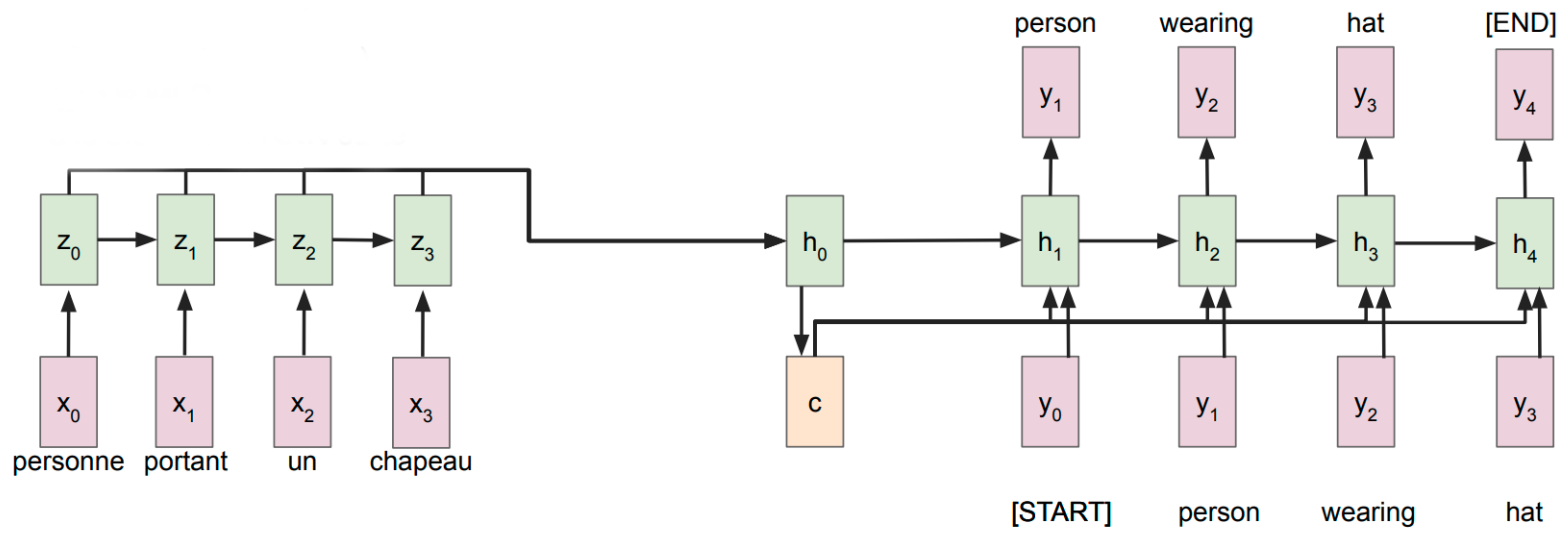
\includegraphics[width=14cm]{images/machinetranslation-noattention.png}
\end{frame}

%%%%%%%%%%%%%%%%%%%%%%%%%%%%%%%%%%%%%%%%%%%%%%%%%%%%%%%%%%%%%%
\begin{frame}{Attention for token-dependent context vectors}
  \centering
  \[\qquad\qquad\qquad\qquad\qquad\mathbf{c}_t = \sum_{n} a_{n}^{(t)}\mathbf{z}_{n}\quad \text{(mul \& add)}\vspace{-10mm}\]
 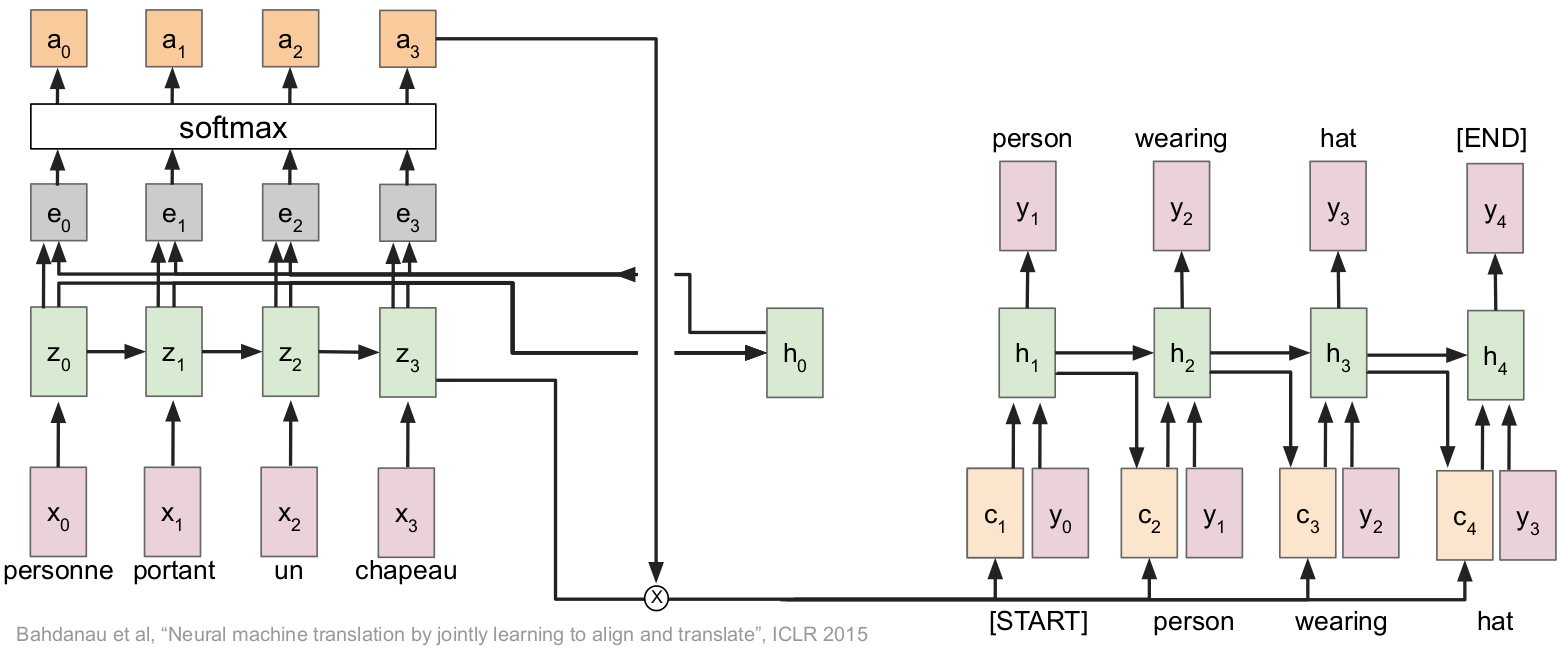
\includegraphics[width=14cm]{images/machinetranslation-attention.png}
\end{frame}

\section{Self-attention}

%%%%%%%%%%%%%%%%%%%%%%%%%%%%%%%%%%%%%%%%%%%%%%%%%%%%%%%%%%%%%%
\begin{frame}{Basic operation: softmax}
Computes some the ``probability of a discrete event'' using:
\[ \textrm{softmax}(\mathbf{z})_j =  \frac{\exp(z_j/\tau)}{\sum_{k=1}^K \exp(z_k/\tau)}, \forall j=1,\ldots,K,\]
 where $\tau$ is referred to as the \textit{temperature}.
\begin{figure}
 \centering
 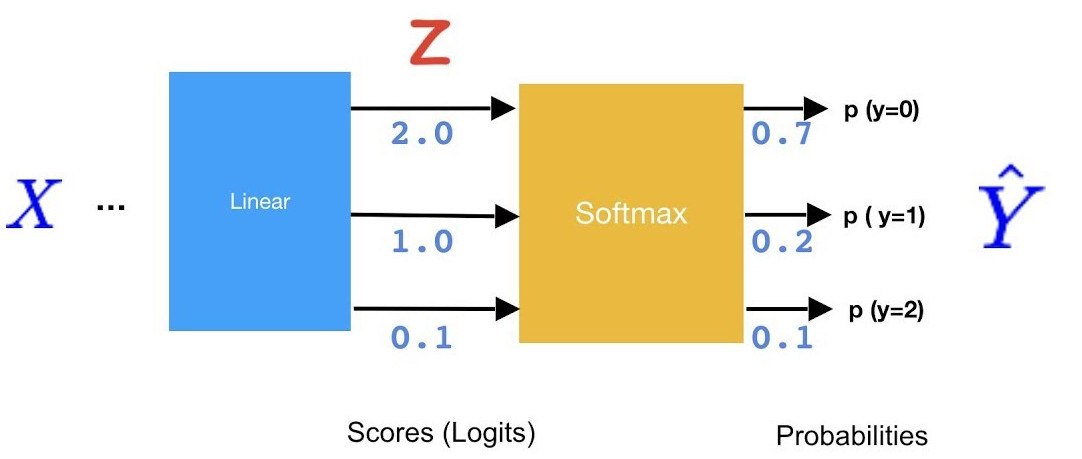
\includegraphics[width=7cm]{images/softmax}
\end{figure}
Softmax is appropriate because you have a limited (attention) budget to distribute. 
 \end{frame}

%%%%%%%%%%%%%%%%%%%%%%%%%%%%%%%%%%%%%%%%%%%%%%%%%%%%%%%%%%%%%%
\begin{frame}{How to compute attention?}
  \begin{columns}
  \begin{column}{0.25\textwidth}
   \begin{flushright}
    \scriptsize Output/context\hspace{4mm}$ $\vspace{-3mm}
   \end{flushright}
   \centering
   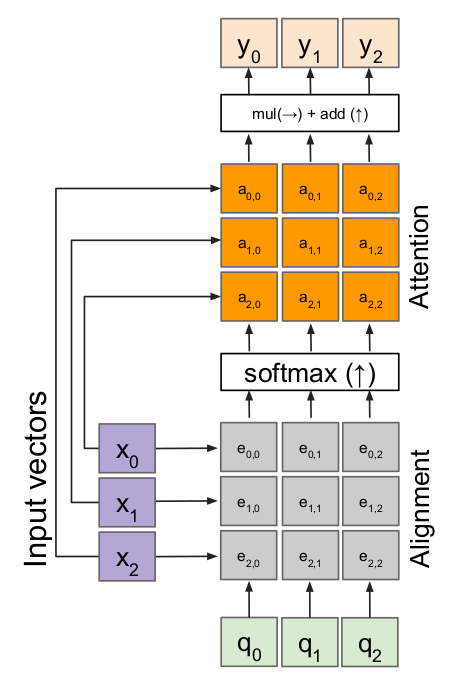
\includegraphics[width=\textwidth]{images/multiple-queries}
  \end{column}
  \begin{column}{0.75\textwidth}
      Interpreted as a query ($\mathbf{q}_m$), key ($\mathbf{x}_n$) and value (same $\mathbf{x}_n$).\\
    {\scriptsize ($\mathbf{q}_m$ and $\mathbf{x}_n$ have the same dimension $D$)}\vspace{5mm}\\

    Different number of queries $M$ than input vectors $N$.\vspace{5mm}\\
    
    Alingment is computed with norm. dot product: $\mathbf{e}_{n,m} = \mathbf{x}_n^\top \mathbf{q}_m / \sqrt{D}$.\vspace{5mm}\\
    
    Attention is computed with softmax: $a_{n,m} = \textrm{softmax}_n(\mathbf{e}_{n,m})$.\vspace{5mm}\\
    
    Output/context is computed with weighted sum: $\mathbf{y}_m = \sum_{n} a_{n,m}\mathbf{x}_{n}$.\vspace{5mm}\\
      
   \textbf{Limitation}: input vectors are both keys and values.
  \end{column}
 \end{columns}
\end{frame}

%%%%%%%%%%%%%%%%%%%%%%%%%%%%%%%%%%%%%%%%%%%%%%%%%%%%%%%%%%%%%%
\begin{frame}{More expressivity!}
  \begin{columns}
  \begin{column}{0.3\textwidth}
   \centering
   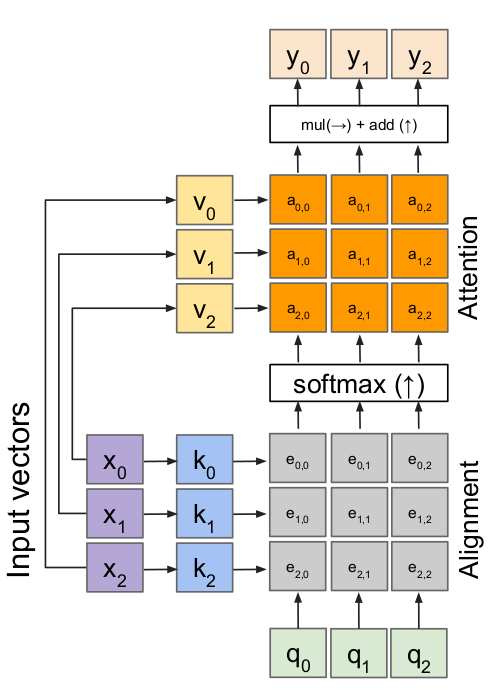
\includegraphics[width=\textwidth]{images/more-expressivity}
  \end{column}
  \begin{column}{0.7\textwidth}
   Add MLP to compute keys and values.\vspace{5mm}\\
   
   Allows for more expressivity, and also to change dimensions.   
   \[\mathbf{k}_n=\textrm{MLP}_k(\mathbf{x}_n) \in \mathbb{R}^{D_k}\]
   \[\mathbf{v}_n=\textrm{MLP}_v(\mathbf{x}_n) \in \mathbb{R}^{D_v}\]
   ($D_k$ should also be the dimension of $\mathbf{q}_m$)\vspace{5mm}\\
   
   But remember that the RNN was initialised from the image/text features: the \textbf{input} features.
   
  \end{column}
 \end{columns}
\end{frame}

%%%%%%%%%%%%%%%%%%%%%%%%%%%%%%%%%%%%%%%%%%%%%%%%%%%%%%%%%%%%%%
\begin{frame}{Self-attention layer}
  \begin{columns}
  \begin{column}{0.3\textwidth}
   \centering
   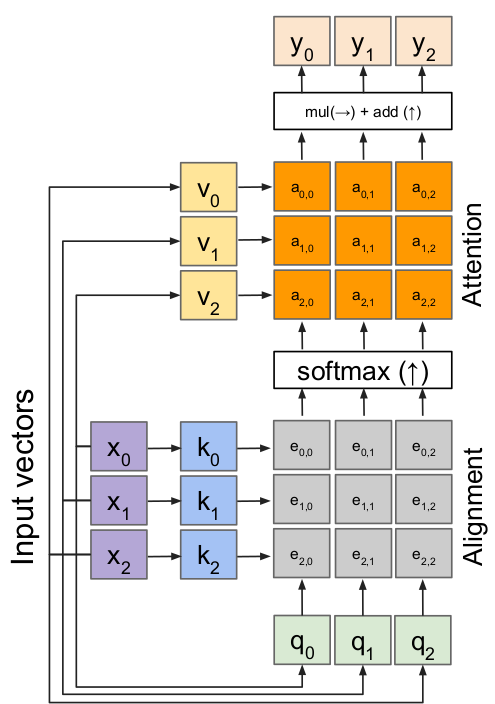
\includegraphics[width=\textwidth]{images/self-attention-layer}
  \end{column}

  \begin{column}{0.7\textwidth}
   Add MLP to compute the queries as well.
   \[\mathbf{q}_n=\textrm{MLP}_q(\mathbf{x}_n) \in \mathbb{R}^{D_k}\]
   ($D_k$ should also be the dimension of $\mathbf{q}_m$)\vspace{5mm}\\
   
   Now we have as many queries as input vectors.\vspace{5mm}\\
   
   This is the well-known \textbf{self-attention} layer, and is the basis of transformers.
  \end{column}
 \end{columns}
\end{frame}


%%%%%%%%%%%%%%%%%%%%%%%%%%%%%%%%%%%%%%%%%%%%%%%%%%%%%%%%%%%%%%
\begin{frame}{Self-attention vs.\ cross-attention}
  \begin{columns}
  \begin{column}{0.3\textwidth}
   \centering
   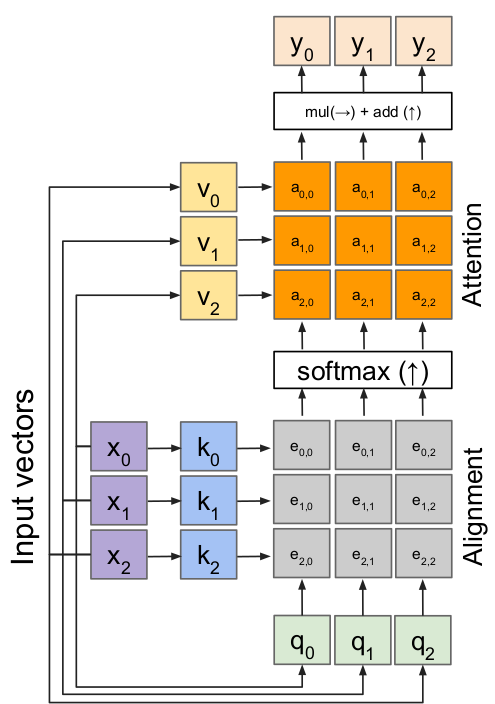
\includegraphics[width=\textwidth]{images/self-attention-layer}
  \end{column}
  \begin{column}{0.35\textwidth}
    Self-attention (left) vs.\ cross-attention (right).\vspace{5mm}
    
    Self-attention: queries, keys and values are computed from the input.\vspace{5mm}
    
    Cross-attention: keys and values are computed from the input, BUT queries come from a different source (usually called memory).\vspace{5mm}
  \end{column}
    \begin{column}{0.3\textwidth}
   \centering
   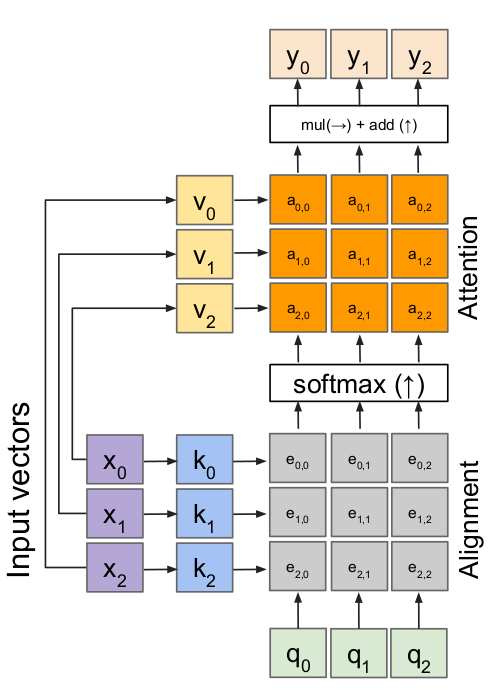
\includegraphics[width=\textwidth]{images/more-expressivity}
  \end{column}
 \end{columns}
\end{frame}

%%%%%%%%%%%%%%%%%%%%%%%%%%%%%%%%%%%%%%%%%%%%%%%%%%%%%%%%%%%%%%
\begin{frame}{Application: image captioning}
 \begin{figure}
  \centering
  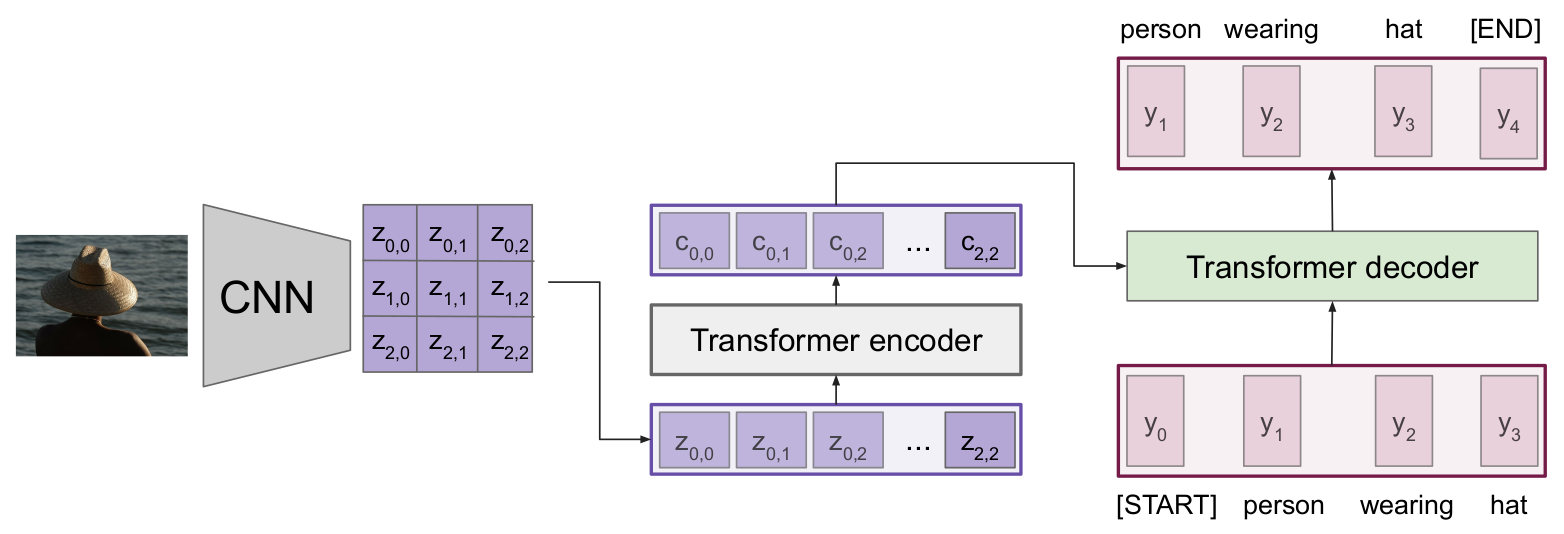
\includegraphics[width=12cm]{images/transformer-overview}
 \end{figure}
 \textbf{Encoder}: uses self-attention to output pixel-dependent context vectors.
 
 \textbf{Decoder}: uses cross-attention to take into account these context vectors, and self-attention to take into account already decoded words.\vspace{4mm}
 
 But what is a transformer?
\end{frame}


\section{Transformers}

%%%%%%%%%%%%%%%%%%%%%%%%%%%%%%%%%%%%%%%%%%%%%%%%%%%%%%%%%%%%%%
\begin{frame}{Improving self-attention}
Main problem of self-attention: permutation invariant!\\
We can reorder the input features (the the output will follow the same permutation).\vspace{5mm}

But data are not permutation-invariant (images, text, audio, ...)
  \begin{columns}
  \begin{column}{0.3\textwidth}
   \centering
   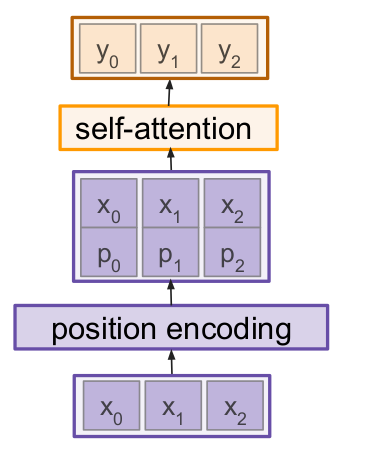
\includegraphics[width=\textwidth]{images/positional-encoding-1}
  \end{column}
  \begin{column}{0.7\textwidth}
   Concatenate positional vectors to features.\vspace{3mm}\\
   
   Design a function $\mathbf{p}_j=f_p(j)$ encoding the position:
   \begin{itemize}
    \item Unique $\mathbf{p}_j$'s.
    \item Distance between time steps independent of length.
    \item Generalise to different lengths.
    \item Deterministic.
   \end{itemize}
  \end{column}
 \end{columns}
\end{frame}

%%%%%%%%%%%%%%%%%%%%%%%%%%%%%%%%%%%%%%%%%%%%%%%%%%%%%%%%%%%%%%
\begin{frame}{Positional encoding}
  \begin{columns}
  \begin{column}{0.3\textwidth}
   \centering
   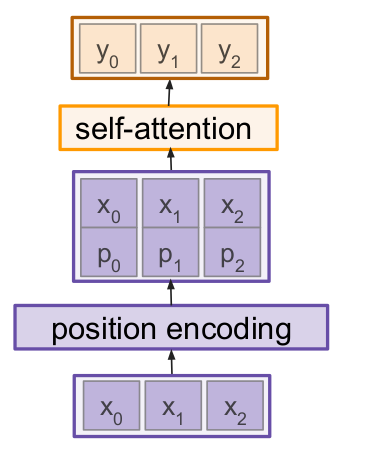
\includegraphics[width=\textwidth]{images/positional-encoding-1}
  \end{column}
  \begin{column}{0.3\textwidth}
    \[f_p(j) = \left(\begin{array}{c} \sin(\omega_1t)\\ \cos(\omega_1t) \\ \sin(\omega_2t)\\ \cos(\omega_2t) \\ \vdots \\ \sin(\omega_{d/2}t)\\\cos(\omega_{d/2}t) \end{array}\right)\in\mathbb{R}^d\]
    \[w_k = (C)^{-2k/d}\]
  \end{column}
  \begin{column}{0.3\textwidth}
   \centering
   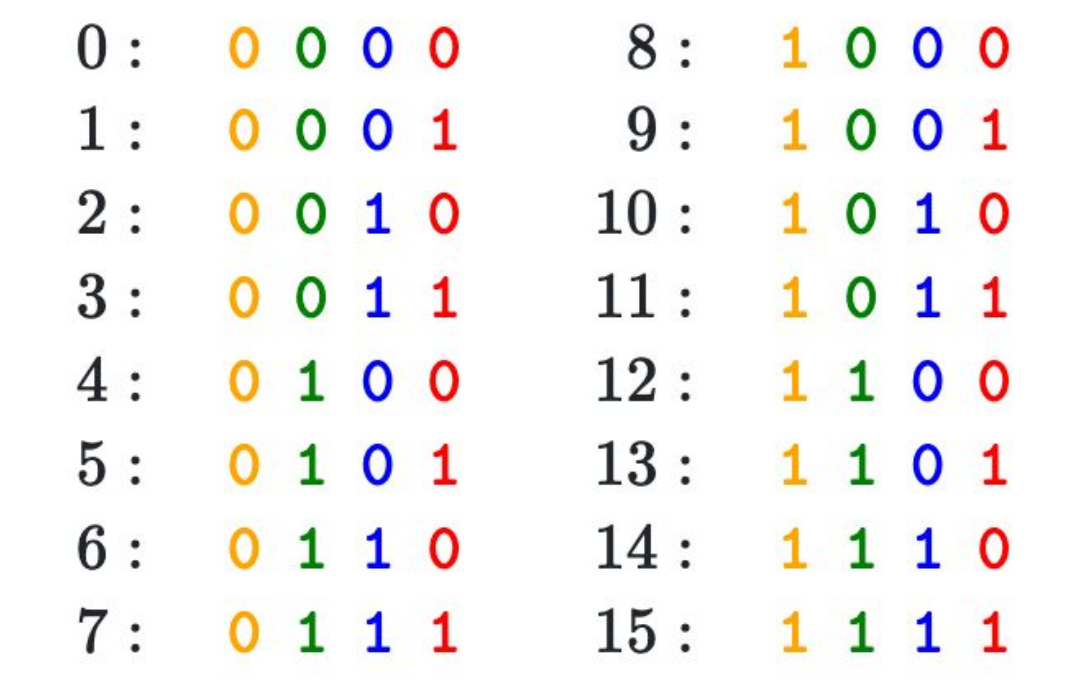
\includegraphics[width=\textwidth]{images/pe-intuition}\vspace{6mm}
   Large $C=10000$ is used.
  \end{column}
 \end{columns}
\end{frame}

%%%%%%%%%%%%%%%%%%%%%%%%%%%%%%%%%%%%%%%%%%%%%%%%%%%%%%%%%%%%%%
\begin{frame}{Other add-ons: masking}
   \begin{columns}
  \begin{column}{0.4\textwidth}
   \centering
   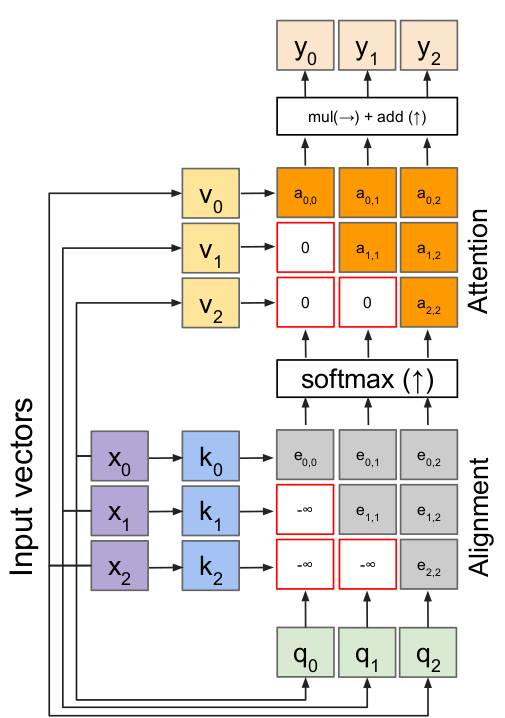
\includegraphics[width=0.75\textwidth]{images/masked-self-attention}
  \end{column}
  \begin{column}{0.7\textwidth}
    Avoid paying attention to the future.\vspace{5mm}\\
    
    Mask-out using the softmax operation.\vspace{5mm}\\
    
    Set the alignment scores to $-\infty$.
  \end{column}
 \end{columns}
\end{frame}

%%%%%%%%%%%%%%%%%%%%%%%%%%%%%%%%%%%%%%%%%%%%%%%%%%%%%%%%%%%%%%
\begin{frame}{Other add-ons: multiple heads}
Intuition: be able to specialise and pay attention to a different feature.
  \begin{figure}
   \centering
   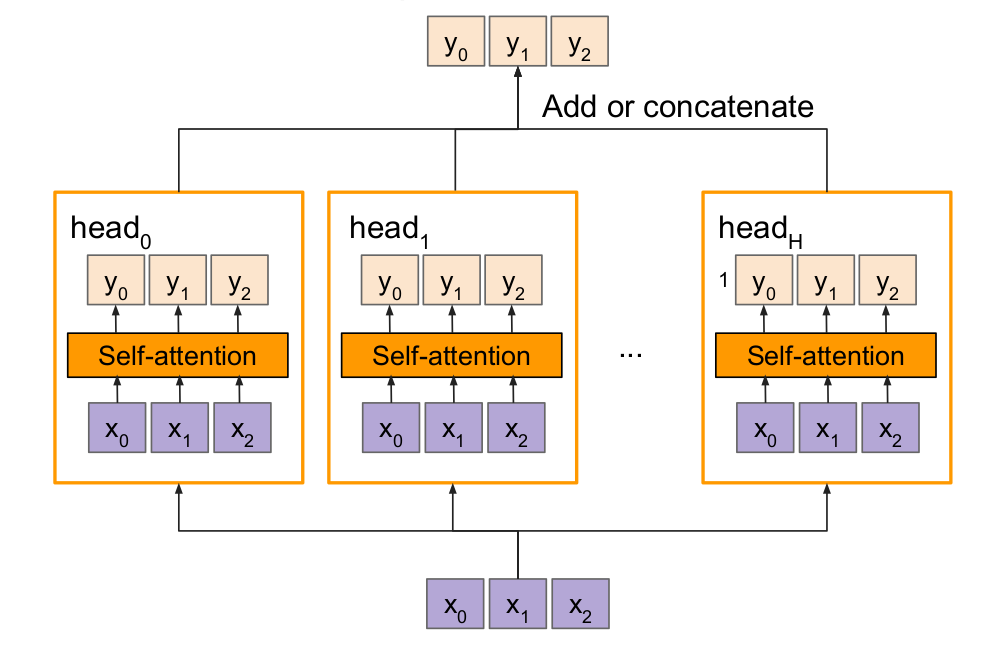
\includegraphics[width=10cm]{images/multi-head-attention}
  \end{figure}
\end{frame}

%%%%%%%%%%%%%%%%%%%%%%%%%%%%%%%%%%%%%%%%%%%%%%%%%%%%%%%%%%%%%%
\begin{frame}{Layer normalisation}
 Remember batch normalisation (left)? We also have layer normalisation (right)!
 \begin{figure}
  \centering
  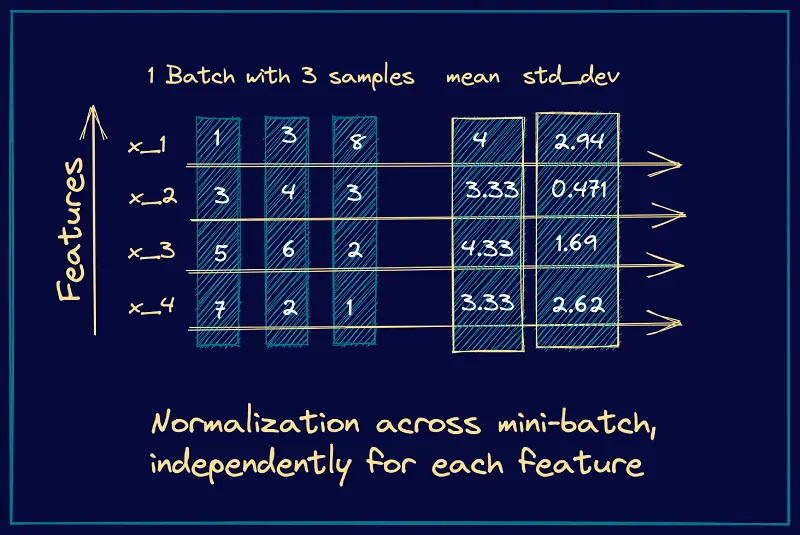
\includegraphics[width=0.45\textwidth]{images/batchnorm.jpg}\hspace{3mm}
  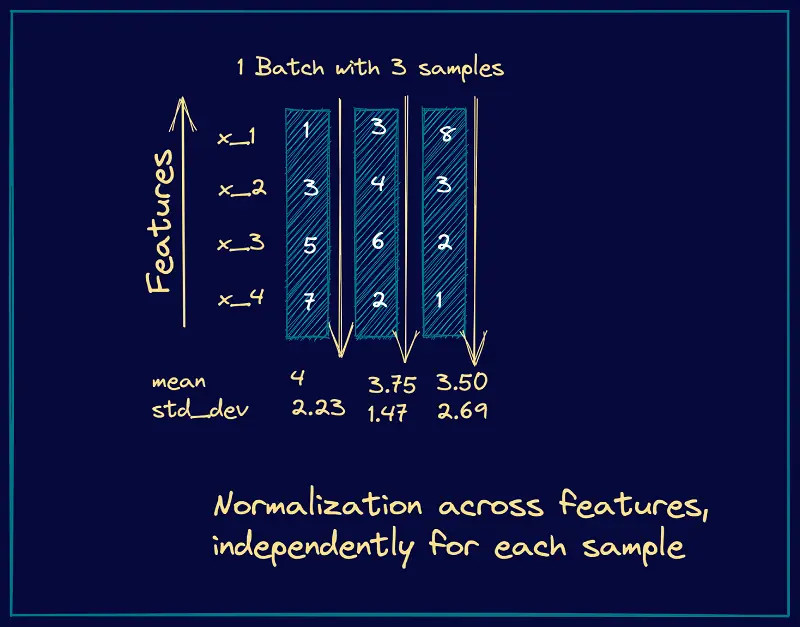
\includegraphics[width=0.385\textwidth]{images/layernorm.jpg}
 \end{figure}
 Instead of normalising each feature with the statistics of the mini-batch, we normalise each channel with the statistics of one sample (does not depend on $N$).
\end{frame}



%%%%%%%%%%%%%%%%%%%%%%%%%%%%%%%%%%%%%%%%%%%%%%%%%%%%%%%%%%%%%%
\begin{frame}{Transformers: encoder}
 \begin{columns}
  \begin{column}{0.5\textwidth}
   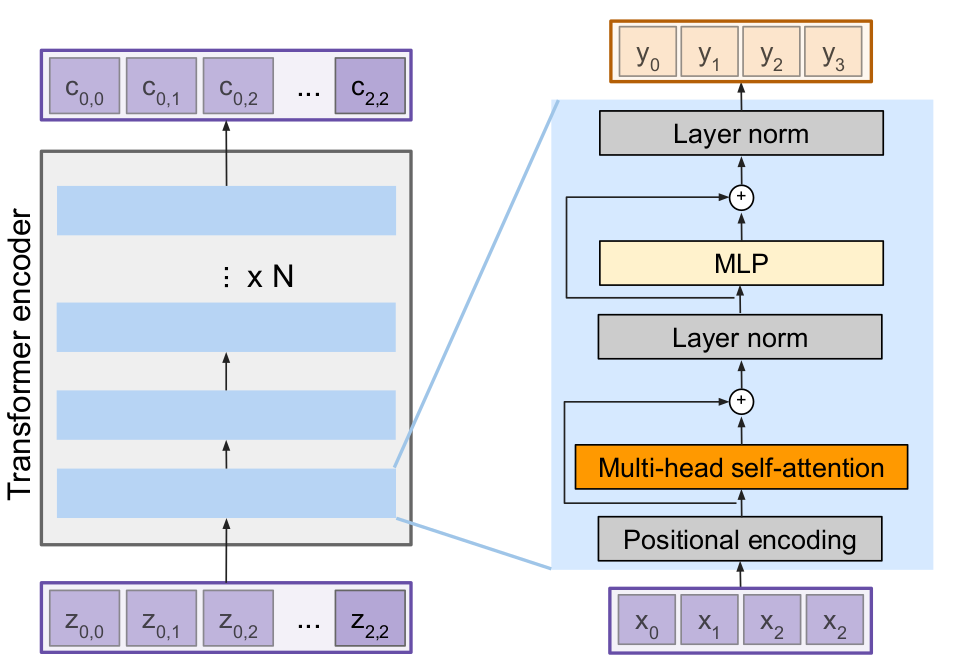
\includegraphics[width=\textwidth]{images/transformer-encoder}
  \end{column}
  \begin{column}{0.5\textwidth}
   \begin{itemize}
    \item Positional encoding, layer normalisation, residual connections and MLP operate \textbf{independently} per each vector.\vspace{3mm}
    \item The only operation combining the information across vectors is the multi-head self-attention.\\
    (Remember that queries, keys and values are all computed from input)
   \end{itemize}
  \end{column}
 \end{columns}

\end{frame}


%%%%%%%%%%%%%%%%%%%%%%%%%%%%%%%%%%%%%%%%%%%%%%%%%%%%%%%%%%%%%%
\begin{frame}{Transformers: decoder}
 \begin{columns}
  \begin{column}{0.5\textwidth}
   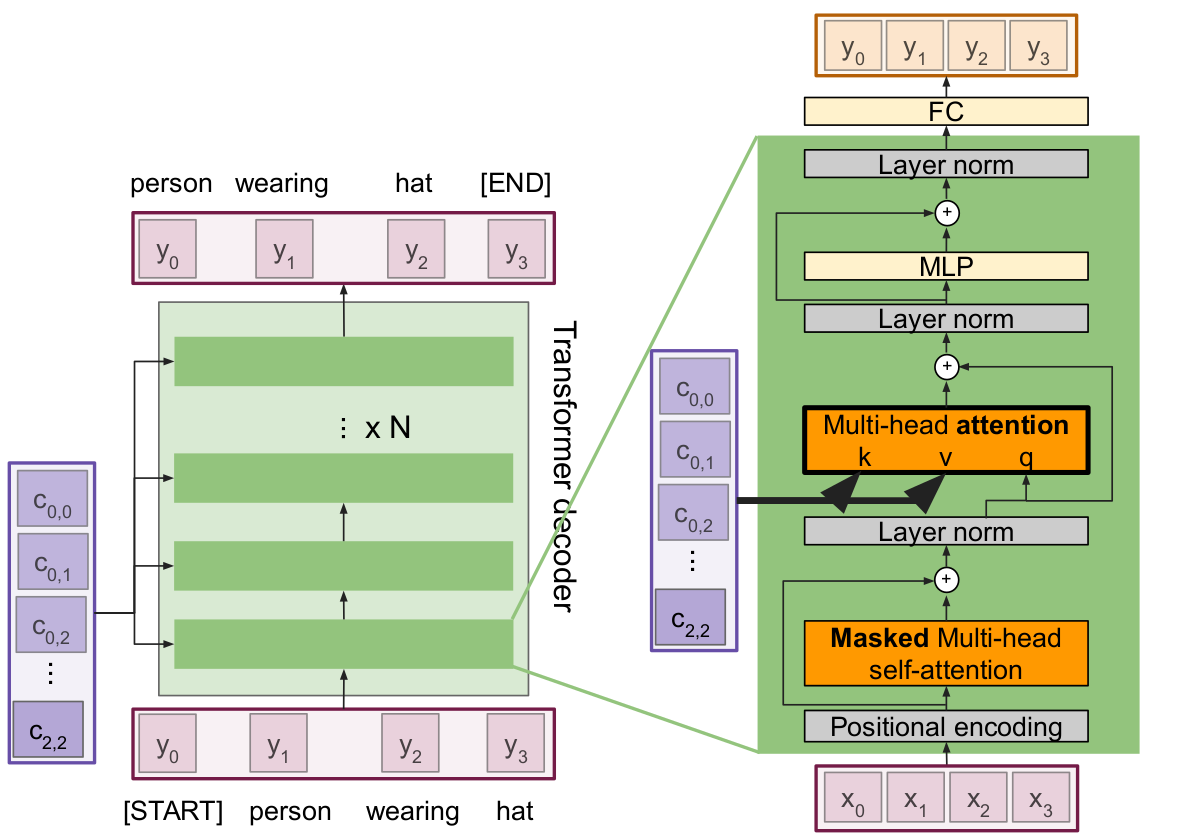
\includegraphics[width=\textwidth]{images/transformer-decoder}
  \end{column}
  \begin{column}{0.5\textwidth}
   \begin{itemize}
    \item Except attention, all operations are query-wise.\vspace{3mm}
    \item Masked self-attention (to avoid looking into the decoded future).\vspace{3mm}
    \item Multi-head attention (to compare the queries with the encoder memory).
   \end{itemize}
  \end{column}
 \end{columns}

\end{frame}

%%%%%%%%%%%%%%%%%%%%%%%%%%%%%%%%%%%%%%%%%%%%%%%%%%%%%%%%%%%%%%
\begin{frame}{Transformers: conclusion}
 \begin{itemize}
  \item Adding attention (to RNN or DNN in general) allows the network to focus on different parts of the input.\vspace{3mm}
  \item The attention layer operates vector-wise, and learns how to pay attention (and to which parts of other vectors).\vspace{3mm}
  \item Transformer are encoder-decoder architectures using self-attention, masked attention and multi-head attention.\vspace{3mm}
  \item They are highly parallelizable (and hence scalable), and yield outstanding performance. They do pose a memory issue.
 \end{itemize}
\end{frame}

%%%%%%%%%%%%%%%%%%%%%%%%%%%%%%%%%%%%%%%%%%%%%%%%%%%%%%%%%%%%%%
\begin{frame}{Examples on image captioning}
Different parts of the image should be used to decide each word.
 \centering
 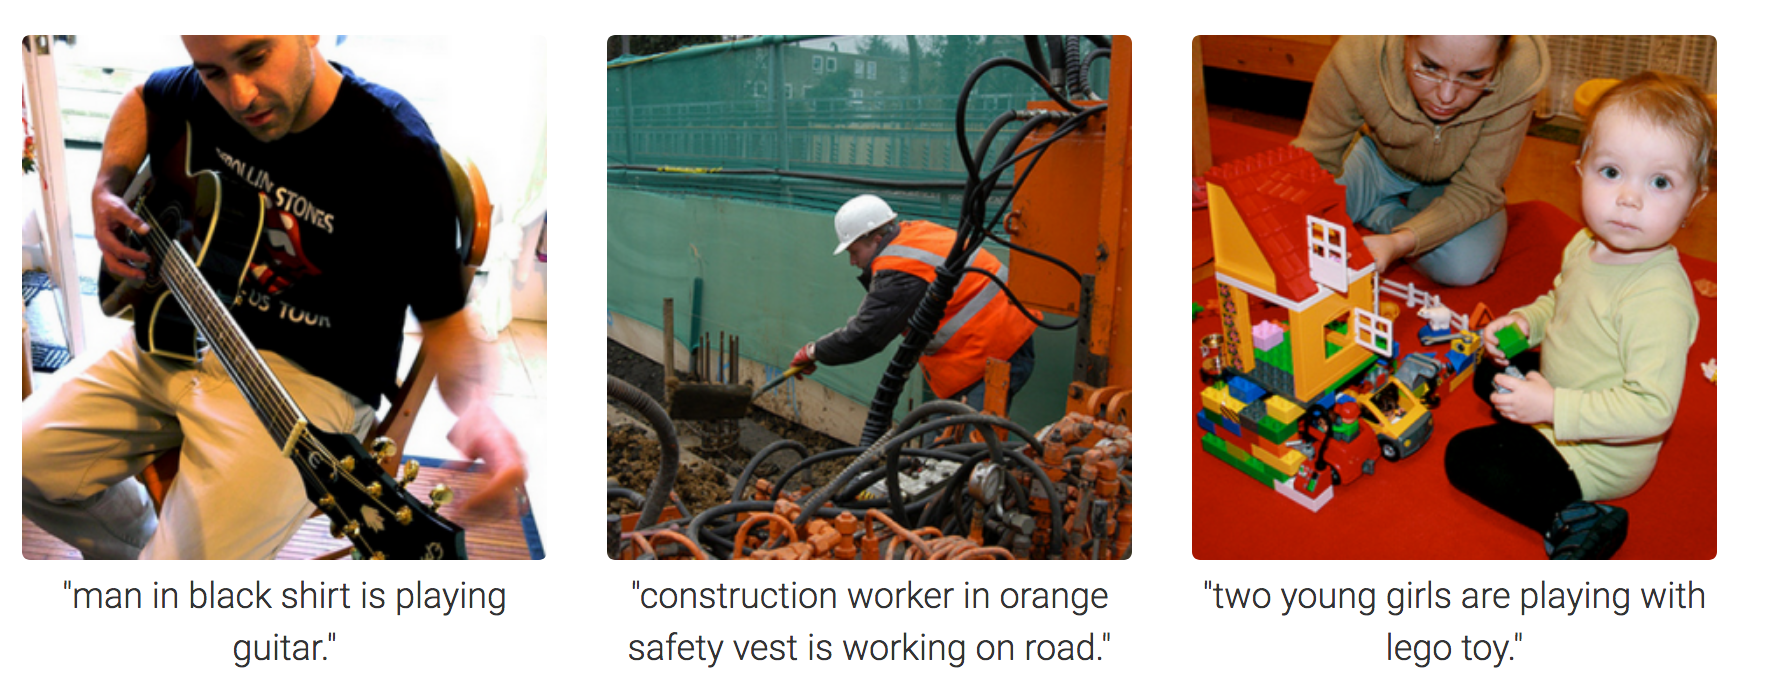
\includegraphics[width=14cm]{images/imagecaptioning.png}
\end{frame}
% 
% %%%%%%%%%%%%%%%%%%%%%%%%%%%%%%%%%%%%%%%%%%%%%%%%%%%%%%%%%%%%%%
% \begin{frame}{First attemp: combine CNN and RNN}
%  \begin{figure}
%   \centering
%   \includegraphics[width=13cm]{images/imagecaptioning-rnn.png}
%  \end{figure}
%  \begin{itemize}
%   \item CNN used to extract features ($H\times W\times D$) and MLP to get the conditioning $c$.
%   \item $c$ is used at ALL time steps to condition the output of the RNN.
%   \item This is \alert{problematic} for very long sequences (even using LSTM).
%  \end{itemize}
% 
% \end{frame}
% 
% %%%%%%%%%%%%%%%%%%%%%%%%%%%%%%%%%%%%%%%%%%%%%%%%%%%%%%%%%%%%%%
% \begin{frame}{Attention: intuition}
%   The idea is to have a different conditioning vector at every time step:
%   \begin{figure}
%     \centering
%     \includegraphics[width=13cm]{images/imagecaptioning-attention.png}
%  \end{figure}
%  These different conditioning vectors should be \textbf{paying attention} to different CNN features.
% \end{frame}
% 
% 
% 
% %%%%%%%%%%%%%%%%%%%%%%%%%%%%%%%%%%%%%%%%%%%%%%%%%%%%%%%%%%%%%%
% \begin{frame}{Attention with RNNs}
%  \begin{columns}
%   \begin{column}{0.5\textwidth}
%    \centering
%    \includegraphics[width=\textwidth]{images/imagecaptioning-attention-1frame}
%   \end{column}
%   \begin{column}{0.5\textwidth}
%     First, alignment scores are computed:
%     \[\mathbf{e}_{t,w,h}=\textrm{MLP}(\mathbf{z}_{w,h},\mathbf{h}_t).\]
%     Second, attention is computed with softmax:
%     \[\mathbf{a}_{t,:,:} = \textrm{softmax}(\mathbf{e}_{t,:,:}).\]
%     Finally, the conditioning vector is computed from the features weighted by attention:
%     \[\mathbf{c}_t = \sum_{w,h} a_{t,w,h}\mathbf{z}_{w,h}\]
%   \end{column}
%  \end{columns}\vspace{2mm}
% 
%  This is applied at every time step, obtaining different attention maps $\mathbf{a}_t$ and different conditioning vectors $\mathbf{c}_t$ $\Rightarrow$ Each token is decoded paying attention to different features.
% \end{frame}

\end{document}

